%auto-ignore
\chapter[DIVE: A Spatiotemporal Progression Model of Brain Pathology]{DIVE: A Spatiotemporal Progression Model of Brain Pathology in Neurodegenerative Disorders}
\label{chapter:dive}

In this chapter I present DIVE, a novel spatiotemporal model of disease progression that I estimates fine-grained spatial patterns of atrophy in the brain. I did the entire work: model development, mathematical derivations (Supplementary section \ref{sec:diveAppendix}), image pre-processing and analysis and wrote the manuscripts. Arman Eshaghi showed me how to perform the image processing with Freesurfer. Daniel Alexander and Marco Lorenzi offered suggestions with modelling and experiment design. All collaborators gave me feedback on the manuscripts.

\section{Publications}
\begin{itemize}
 \item R. V. Marinescu, A. Eshaghi, M. Lorenzi, A. L. Young, N. P. Oxtoby, S. Garbarino, T. J. Shakespeare, S. J. Crutch and D. C. Alexander, A Vertex Clustering Model for Disease Progression: Application to Cortical Thickness Images, Information Processing in Medical Imaging, 2017
 \item R. V. Marinescu, A. Eshaghi, M. Lorenzi, A. L. Young, N. P. Oxtoby, S. Garbarino, S. J. Crutch, D. C. Alexander, DIVE: A spatiotemporal progression model of brain pathology in neurodegenerative disorders, NeuroImage, 2019.
\end{itemize}


\section{Introduction}
\label{sec:diveInt}

Current image-based disease progression models, such as those presented in section \ref{sec:bckSca}, estimate the evolution of the disease using a small set of biomarkers corresponding to pre-defined regions-of-interest (ROI). This ROI parcellation is usually coarse and doesn't allow one to find spatially dispersed patterns of atrophy. While spatiotemporal longitudinal models have already been demonstrated \cite{derado2010modeling, hyun2016stgp, lorenzi2015efficient}, these models regress against pre-defined sets of covariates such as age, time since baseline or clinical markers. This is problematic because, age-based alignment of subjects assumes all subjects have the same age of disease onset, while for time since baseline, its relationship with disease onset is unknown. Similarly, clinical markers are noisy, biased, suffer from floor/ceiling and training effects, are not sensitive in pre-symptomatic phases, and have low test-retest reliability \cite{johnson2012brain}.  Recently, some spatiotemporal models that estimate subject-specific time-shifts have been developed \cite{bilgel2016multivariate,koval2017statistical}. However, these models generally cannot recover dispersed and disconnected pathological patterns, because they assume voxel measurements correlate based on spatial distance, either through a distance function or distance from control points. However, spatially dispersed pathological patterns have been observed in AD and related dementias and are hypothesised to appear due to the interaction of pathology with brain networks \cite{seeley2009neurodegenerative}. Discovering such fine-grained patterns could allow one to understand underlying mechanisms of pathology propagation along these networks. However, a spatiotemporal disease progression model that allows recovery of dispersed and disconnected atrophy patterns present in AD, is not currently available. 

In this work, we present DIVE: Data-driven Inference of Vertexwise Evolution. DIVE is a novel disease progression model with single vertex resolution that makes only weak assumptions on spatial correlation. In contrast to approaches which model temporal trajectories for a small set of biomarker measures based on a priori defined ROIs, DIVE models temporal trajectories for each vertex on the cortical surface. DIVE combines unsupervised learning and disease progression modelling to identify clusters of vertices on the cortical surface that show a similar trajectory of brain pathology over a particular patient cohort. This formulation enables us to estimate a fine-grained spatial distribution of pathology and also provides a novel parcellation of the brain based on temporal change. 

We first test DIVE on synthetic data and show that the model can recover known biomarker trajectories and time-shifts. We then demonstrate the model on both MRI and PET data from two cohorts: the Alzheimer's Disease Neuroimaging Initiative (ADNI) and the Dementia Research Centre (DRC), UK. We use the model to reveal spatiotemporal patterns of pathology to a much finer resolution than previous models and demonstrate the ability to assign subjects to stages that predict progression. Finally, we validate DIVE in terms of how robust are the estimated pathology patterns and how well the disease progression scores correlate with cognitive tests. Code for DIVE is available online: \url{https://github.com/mrazvan22/dive}.


\section{Methods}
\label{sec:diveMet}

In this section we describe the mathematical formulation of DIVE (section \ref{sec:diveMod}), then we show how to fit the model using Expectation Maximisation (section \ref{sec:diveFit}) and we describe further implementation details of the algorithm (section \ref{sec:diveImplem}). Afterwards, we outline the synthetic data-generation process (section \ref{sec:diveSimulations}) for testing the model in the presence of ground truth, as well as the pipeline for pre-processing the ADNI and DRC datasets (section \ref{sec:diveDataAcquis}).

\begin{figure}
 \centering
 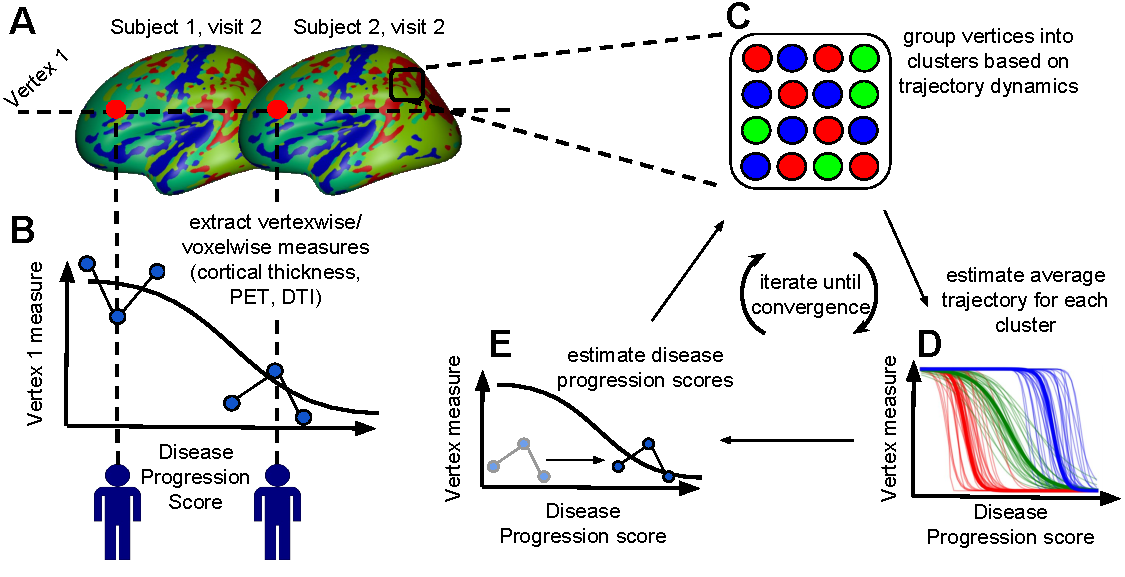
\includegraphics[width=\textwidth]{images/vwdpm_diagram.pdf}
 \caption[Diagram of the proposed DIVE model.]{Diagram of the proposed DIVE model. DIVE assumes that biomarkers of pathology (e.g. cortical thinning) can be measured at many vertices (i.e. locations) on the cortical surface (A), where each vertex has a distinct trajectory of change during disease progression (B). In (B), each individual has measurements for vertex 1 at three visits. DIVE assigns to every cortical vertex one of a small set of temporal trajectories describing the change in some image-based measurement (e.g. cortical thickness, amyloid PET, DTI fractional anisotropy measures) from beginning to end of the disease progression. The estimation process simultaneously estimates the set of clusters, the trajectory defining each cluster, and the position of each subject along the trajectories, which are defined on a common timeline. The process iterates assignment of each vertex to clusters (red, green and blue in this diagram) (C), estimation of the trajectory in each cluster (D) and estimation of the disease progression score (location along trajectory) for  each subject (E), all within an Expectation-Maximisation framework, until convergence. In particular, (E) shows how the disease progression score, which is initially set to the individual's age, converges to the disease stage of the subject. Diagram made by me. }
 \label{fig:diveDiagram}
\end{figure}

\subsection{DIVE Model}
\label{sec:diveMod}

Figure \ref{fig:diveDiagram} illustrates the DIVE aims and implementation. DIVE input measures are vertexwise or voxelwise biomarker measures in the brain (Fig \ref{fig:diveDiagram}\textcolor{blue4}{A}), such as cortical thickness or amyloid load. A vertex is a location on the cortical surface at which a biomarker of pathology is quantifiable (e.g. cortical thickness). For each vertex on the cortical surface (or voxel in the 3D brain volume), we estimate a unique trajectory along the disease progression timeline (Fig \ref{fig:diveDiagram}\textcolor{blue4}{B}), while also estimating subject/visit-specific disease progression scores (i.e. disease stages). We do that by grouping vertices with similar biomarker trajectories into clusters (Fig \ref{fig:diveDiagram}\textcolor{blue4}{C}), and we estimate a representative trajectory for every cluster (Fig \ref{fig:diveDiagram}\textcolor{blue4}{D}). Each trajectory is a function of subject-/visit-specific disease progression scores (DPS) (Fig \ref{fig:diveDiagram}\textcolor{blue4}{E}). The DPS depends linearly on the time since baseline visit, but with subject-specific slope and intercept.

\subsection{Modelling Subject-specific Parameters}

The disease progression score $s_{ij}$ for subject $i$ at visit $j$ is a latent variable denoting the current disease stage of the subject at this visit. It  defined as a linear transformation of time since baseline measurement $t_{ij}$ (in years):

\begin{equation}
\label{eq:dps_vwdpm}
 s_{ij} = \alpha_i t_{ij} + \beta_i
\end{equation}
where $\alpha_i$ and $\beta_i$ represent the speed of progression and time shift (i.e. disease onset) of subject $i$ respectively. 

\subsection{Modelling Biomarker Trajectory for a Single Vertex}

DIVE assumes that the biomarker measure at each vertex on the cortical surface follows a sigmoidal trajectory $f(s ; \theta)$ over the disease progression score $s$ and with parameters $\theta$. We choose a parametric sigmoid function because it is a parsimonious parametric model that offers better fit compared to linear models, is monotonic, and can account for floor and ceiling effects \cite{caroli2010dynamics, sabuncu2011dynamics}. We also assume that vertices are grouped into $K$ clusters and we model a unique trajectory for each cluster $k \in {1, ... , K}$, which will be referred to as cluster trajectories. The sigmoidal function $f(s; \theta_k)$ for cluster $k$ is defined as: 

\begin{equation}
\label{eq:dps_vwdpm2}
 f(s;\theta_k) = \frac{a_k}{1+exp(-b_k(s-c_k))} + d_k
\end{equation}
where $s$ is the disease progression score from Eq. \ref{eq:dps_vwdpm} and $\theta_k = [a_k, b_k, c_k, d_k]$ are parameters controlling the shape of the trajectory -- $d_k$ and $d_k + a_k$ represent the lower and upper limits of the sigmoidal function, $c_k$ represents the inflection point and $a_k b_k/4$ represents the slope at the inflection point. 

For a given subject $i$ at visit $j$, the value $V_l^{ij}$ of its biomarker measurement at vertex $l$ is a random variable that has an associated discrete latent variable $Z_l \in [1, ... , K]$ denoting the cluster it was generated from. The value of $V_l^{ij}$ given that it was generated from cluster $Z_l$ can be modelled as:

% model for one voxel and label
\begin{equation}
\label{eq:dps_vwdpm3}
 p(V_l^{ij} | \alpha_i, \beta_i, \theta_{Z_l}, \sigma_{Z_l}, Z_l) = N(V_l^{ij} | f(\alpha_i t_{ij} + \beta_i | \theta_{Z_l}), \sigma_{Z_l})
\end{equation}
where $N(V_l^{ij} | f(\alpha_i t_{ij} + \beta_i | \theta_{Z_l}), \sigma_{Z_l})$ represents the probability density function (pdf) of the normal distribution that models the measurement noise along the sigmoidal trajectory of cluster $Z_l$, having variance $\sigma_{Z_l}$. Next, we assume the measurements from different subjects are independent, while the measurements from the same subject $i$ at different visits $j$ are linked using the disease progression score from equation \ref{eq:dps_vwdpm}. Moreover, we also assume a uniform prior on $Z_l$. This gives the following model:

% all subj are independent
\begin{equation}
\label{eq:dps_vwdpm4}
 p(V_l, Z_l | \alpha, \beta, \theta, \sigma) = \prod_{(i,j) \in I} N(V_l^{ij} | f(\alpha_i t_{ij} + \beta_i | \theta_{Z_l}), \sigma_{Z_l})
\end{equation}
where $I = {(i,j)}$ represents the set of all the subjects $i$ and their corresponding visits $j$. Furthermore, $V_l = [V_l^{ij} | (i,j) \in I]$ is the 1D array of all the values for vertex $l$ across every subject and corresponding visit. Vectors $\alpha = [\alpha_1, \dots, \alpha_S]$ and $\beta = [\beta_1, \dots, \beta_S]$, where $S$ is the number of subjects, denote the stacked parameters for the subject shifts. If a subject $i$ has multiple visits, these visits share the same parameters $\alpha_i$ and $\beta_i$. Vectors $\theta = [\theta_1, \dots, \theta_K]$ and $\sigma = [\sigma_1, \dots, \sigma_K]$, with $K$ being the number of clusters, represent the stacked parameters for the sigmoidal trajectories and measurement noise specific to each cluster.

Due to our main motivation of modelling population trajectories and in order to ensure robustness and identifiability, we did not add random effects to the trajectories of specific subjects.

\subsection{Modelling Biomarker Trajectories for all Vertices}

So far we have a model for only one vertex on the brain surface. We therefore extend the formulation to all the vertices by assuming all these vertex measurements are spatially independent, giving the complete data likelihood:

% all vertices are independent
\begin{equation}
\label{eq:dps_vwdpm5}
 p(V, Z | \alpha, \beta, \theta, \sigma) = \prod_l^L \prod_{(i,j) \in I} N(V_l^{ij} | f(\alpha_i t_{ij} + \beta_i | \theta_{Z_l}), \sigma_{Z_l})
\end{equation}
where $V = [V_1, \dots, V_L]$, $Z = [Z_1, \dots, Z_L]$, $L$ being the total number of vertices on the cortical surface. The formulation so far assumes spatial independence between measurements in different vertices, but in section \ref{sec:diveSpatialCorr} the model is extended to capture spatial correlations. The full joint distribution is given by:

\begin{equation} \label{eq21}
  p(V, Z, \alpha, \beta, \theta, \sigma) = p(V, Z | \alpha, \beta, \theta, \sigma) p(\alpha, \beta, \theta, \sigma)
\end{equation}
where $p(\alpha, \beta, \theta, \sigma)$ is an informative prior on the model parameters defined as follows: 
\begin{equation} \label{eq1}
\begin{split}
 p(V, Z, \alpha, \beta, \theta, \sigma) & = \prod_{i} p(\alpha_i) p(\beta_i)\\
 p(\alpha_i) & \sim \Gamma(\alpha_{shape}, \alpha_{rate})\\
 p(\beta_i) & \sim N(\beta_{mean}, \beta_{std})\\
\end{split}
\end{equation}
where $\alpha_{shape}$, $\alpha_{rate}$, $\beta_{mean}$, $\beta_{std}$ are a-priori defined hyperparameters. The informative priors on the subject-specific parameters help ensure model identifiability, as the model otherwise has two extra degrees of freedom. Such informative priors on $\alpha_i$ and $\beta_i$ also help deal with singularities in the objective functions of $\alpha_i$ and $\beta_i$ when the biomarker trajectories are flat.

We get the final model log likelihood for incomplete data by marginalising over the latent variables $Z$:
\begin{equation}
\label{eq:dps_vwdpm6}
 p(V|\alpha, \beta, \theta, \sigma) = \prod_{l=1}^L \sum_{k=1}^K p(Z_l = k) \prod_{(i,j) \in I} N(V_l^{ij} | f(\alpha_i t_{ij} + \beta_i | \theta_k), \sigma_k)
\end{equation}

Throughout the article, we will use the shorthand $z_{lk} = p(Z_l = k)$.

\subsection{Modelling Spatial Correlation}
\label{sec:diveSpatialCorr}

The version of the model presented so far assumes spatial independence between vertex measurements. However, the regional organisation of the cortex suggests we would expect spatial correlation\footnote{By correlation here we mean that these vertex measurements are not statistically independent} of the vertex measurements. More precisely, measures of cortical thickness or other modalities are often similar in neighbouring vertices on the cortical surface and likely belong to the same cluster. DIVE can be easily extended to include mild spatial constraints on the correlation of vertex measurements via a Markov Random Field (MRF), which encourages neighbouring vertices to have the same corresponding cluster. We hypothesise that incorporating such constraints should reduce the effects of noise and produce a more stable clustering. However, this does not model correlation between the actual vertex values, but only between the latent variables $Z_l$, i.e. the cluster membership of each vertex. The MRF thus has the advantage of not requiring the use of huge covariance matrices, which are otherwise needed if we want to model correlation of vertex values directly. Moreover, in contrast to previous methods that use correlation based on spatial distance \cite{bilgel2016multivariate,koval2017statistical}, we use neighbourhood correlations, which allow us to estimate fine-grained spatial patterns of pathology. With the MRF, the full-data likelihood function of the model now becomes:

\begin{equation}
 p(V, Z | \alpha, \beta, \theta, \sigma, \lambda) = \prod_l^L \left[ \prod_{(i,j) \in I} N(V_l^{ij} | f(\alpha_i t_{ij} + \beta_i | \theta_{Z_l}), \sigma_{Z_l}) \prod_{l_2 \in N_l} \Psi (Z_{l}, Z_{l_2}) \right]
\end{equation}

where $\Psi(Z_l, Z_{l2})$ is a clique term representing the likelihood of a neighbouring vertex $l_2$ to have similar label with vertex $l$. The formula for the clique term is:

\begin{equation}
 \Psi (Z_{l}=k, Z_{l_2}=k_2) = 
 \begin{cases}
  exp(g(\lambda)) & \text{if } k = k_2\\
  exp(-h(\lambda)) & \text{otherwise}
 \end{cases}
\end{equation} 

where $\lambda$ is a parameter controlling how much to penalise neighbouring vertices that belong to distinct clusters, and $g$ and $h$ are positive, monotonic functions over the $\lambda>0$ range. We choose $g(\lambda)=\lambda$ and $h(\lambda)=\lambda^2$, which results in a concave objective function for $\lambda$, ensuring that it can later be optimised (see M-step).

Therefore, the model parameters that need to be estimated are $M = [\alpha, \beta, \theta, \sigma, \lambda]$ where $\alpha$ and $\beta$ are the subject specific shifting parameters, $\theta$ and $\sigma$ are the cluster specific trajectory and noise parameters and $\lambda$ is the clique parameter denoting the penalisation of spatially non-smooth assignments of latent variables $Z$. 

\subsection{Fitting the Model using Generalised Expectation-Maximisation}
\label{sec:diveFit}

We choose to fit our model using Expectation-Maximisation (EM), because it offers a fast convergence given the large number of parameters that need to be estimated and the huge dimensionality of relevant datasets (e.g. 1973 subjects x 163,842 vertices in ADNI). In the next two sections we outline the E-step and M-step. While both of these steps have no closed-form solution, we will solve them using numerical optimisation, which only results in an increase in the objective function at each iteration. However, the EM algorithm is still guaranteed to converge, and this approach is called Generalised EM \cite{bishop2007pattern}.

Algorithm \ref{fig:algo_vwdpm} shows the model fitting procedure using the EM algorithm. The procedure first initialises (line 1) some parameters required to start the EM algorithm: the subject parameters $\alpha$ and $\beta$ and the latent parameters $z_{lk}$ which represent the assignment of vertices to clusters. In the M-step, the method updates the trajectories of each cluster (lines 4-6), the subjects-specific parameters (line 9) and the clique penalty term $\lambda$ (line 17). In the E-step, the method computes $z_{lk}$ (line 18) using previously defined functions that compute $z_{lk}$ given a fixed $\lambda$ (line 14).

\begin{figure}
\begin{algorithm}[H]
 Initialise $\alpha^{(0)}$, $\beta^{(0)}$, $z_{lk}^{(0)}$ \\
  \While{$\theta$, $\sigma$, $\alpha$, $\beta$ or $z_{lk}$ not converged}{
   \tcp*[l]{M-step 1: For each cluster, optimise its trajectory}
    \For{$k=1$ to $K$}{
      ${\theta_k^{(u)} = \argmin_{\theta_k} \sum_{l=1}^L z_{lk}^{(u-1)} \sum_{(i,j) \in I} (V_l^{ij} - f(\alpha_i^{(u-1)} t_{ij} + \beta_i^{(u-1)} | \theta_k))^2  - log\ p(\theta_k)}$\\
      $\theta_k^{(u)} = \mbox{make\_identifiable}(\theta_k^{(u)})$\\
      ${ \left(\sigma_k^{(u)}\right)^2 = \frac{1}{|I|} \sum_{l=1}^L z_{lk}^{(u-1)} \sum_{(i,j) \in I} (V_l^{ij} - f(\alpha_i^{(u-1)} t_{ij} + \beta_i^{(u-1)} | \theta_k^{(u)}))^2 - log\ p(\sigma_k)}$
    }
     \tcp*[l]{M-step 2: For each subject, optimise its time shift $\alpha_i$ and progression speed $\beta_i$}
    \For{$i=1$ to $S$}{
    \footnotesize
      ${\alpha_i^{(u)}, \beta_i^{(u)} = \argmin_{\alpha_i, \beta_i}  \left[ \sum_{l=1}^L \sum_{k=1}^K \frac{z_{lk}^{(u-1)}}{2 \left(\sigma_k^{(u)}\right)^2 } \sum_{j \in I_i} (V_l^{ij} - f(\alpha_i t_{ij} + \beta_i | \theta_k^{(u)}))^2\right] - log\ p(\alpha_i, \beta_i)}$
    \normalfont
    }
   \tcp*[l]{E-step 1: Define functions $\zeta_{lk}(\lambda)$ computing $z_{lk}$, the probability of vertex $l$ being assigned to cluster $k$, given fixed $\lambda$}
  \For{$l = 1$ to $L$}{
    \For{$k = 1$ to $K$}{
      \tcp*[l]{Pre-compute data fit terms $D_{lk}$}
      $D_{lk} = -\frac{1}{2}log\ (2 \pi \left(\sigma_k^{(u)}\right)^2) |I| - \frac{1}{2\left(\sigma_k^{(u)}\right)^2} \sum_{i,j \in I} (V_l^{ij} - f(\alpha_i^{(u)} t_{ij} + \beta_i^{(u)} | \theta_k^{(u)}))^2$\\
%       \tcp*[l]{Function $\zeta_{lk}(\lambda)$ computes $z_{lk}$ for a given $\lambda$}
      $ \zeta_{lk}(\lambda) \approx exp \left( D_{lk} +   \sum_{l_2 \in N_l} log\ \left[ exp(-\lambda^2) + z_{l_2k}^{(u-1)} (exp(\lambda) - exp(-\lambda^2)) \right] \right) $

    }
  }
%   $\Omega(\lambda) = $
  \tcp*[l]{M-step 3: optimise clique term $\lambda$ using above definitions in E-step 1}
%   $ \lambda^{(u)} = \argmax_{\lambda}\ \sum_{l=1}^L \sum_{k=1}^K \zeta_{lk}(\lambda) D_{lk} \  + \lambda \sum_{l = 1}^{L} \sum_{k}^K \sum_{l_2 \in N_l}  \zeta_{lk}(\lambda) \zeta_{l_2 k}(\lambda)\  + (-\lambda^2) \sum_{l = 1}^{L} \sum_{k}^K \sum_{l_2 \in N_l} \zeta_{lk}(\lambda) (1- \zeta_{l_2 k}(\lambda))   $\\
$ \lambda^{(u)} = \argmax_{\lambda}\ \sum_{l=1}^L \sum_{k=1}^K \zeta_{lk}(\lambda) \left[  D_{lk} \  + \lambda \sum_{l_2 \in N_l}  \zeta_{l_2 k}(\lambda)\  -\lambda^2 \sum_{l_2 \in N_l} (1- \zeta_{l_2 k}(\lambda))  \right]  $\\
  
  \tcp*[l]{E-step 2: Compute next $z_{lk}$ using the best $\lambda$}
  $z_{lk}^{(u)} = \zeta_{lk}(\lambda^{(u)})$
  }

  $\alpha_i^{(u)} = \frac{\alpha_i^{(u)}}{\sigma_N}, \beta_i^{(u)} = \frac{\beta_i^{(u)} - \mu_N}{\sigma_N}$   \tcp*[l]{Re-scale subject shifts}
%  }
\end{algorithm}
\caption[The DIVE parameter estimation algorithm.]{The DIVE parameter estimation algorithm. The algorithm, based on Expectation-Maximisation, iteratively optimises the assignment of vertices to clusters (E-step) and the parameters for the biomarker trajectories and subject time-shifts (M-step). }
\label{fig:algo_vwdpm}
\end{figure}
\subsubsection{E-step}

In the Expectation step, at iteration $u$ we seek an estimate of $p(Z | V, M^{(u-1)})$, given the current estimates of the parameters $M^{(u-1)} =[ \theta_k^{(u-1)}, \sigma_k^{(u-1)}, \alpha_i^{(u-1)}, \beta_i^{(u-1)}, \lambda_i^{(u-1)}]$. We perform this using Iterated Conditional Modes \cite{bishop2007pattern}, which performs coordinate-wise gradient ascent. This works by conditioning the clique terms Z on the values of Z from the previous iterations.  This approximation gives the following factorisable likelihood:

\begin{equation}
\label{eq:e_approx}
 p(Z | V, \Mu^{(u-1)}) \approx \prod_l^L \mathbb{E}_{Z_{N_l}^{(u-1)}|V_l, M} \left[ p(Z_l|V_l, \Mu, Z_{N_l}^{(u-1)}) \right]
\end{equation}

The factorised form allows for tractable computation and memory storage of $p(Z)$. Let $z_{lk}(u) = p(Z_l = k | V_l, M^{(u-1)},Z^{(u-1)})$. After simplifications we reach the following update rule:

\begin{equation}
\label{eq:e-step}
\begin{split}
 log\ z_{lk}^{(u)} \propto D_{lk}+ \left[ \sum_{l_2 \in N_l} log\ \left[ exp(-\lambda^2) + z_{l_2k}^{(u-1)} (exp(\lambda) - exp(-\lambda^2)) \right] \right]
\end{split}
\end{equation}
where the data-fit term $D_{lk}$ has the following form:

\begin{equation}
\label{eq:e-step_Dlk}
D_{lk} = -\frac{log\ (2 \pi \sigma_k^2) |I|}{2} - \sum_{i,j \in I}  \frac{1}{2\sigma_k^2}(V_l^{ij} - f(\alpha_i t_{ij} + \beta_i | \theta_k))^2 
\end{equation}

The full derivation is given in Supplementary section \ref{sec:diveEmDerivAppendix}. In order to enable optimisation over $\lambda$, a final modification of this step is performed, by considering $z_{lk}$ to be functions $\zeta_{lk}(\lambda)$ over $\lambda$. This results in the update equation from Alg. \ref{fig:algo_vwdpm}, line 18 which is based on pre-defined terms on lines 13-14. 


\subsubsection{M-step}

In the Maximisation step we try to estimate the model parameters $M = (\alpha, \beta, \theta, \sigma, \lambda)$ that maximise $E_{Z|V,M^{(u-1)}}[log\ p(V,Z|M)]$. We cannot simultaneously optimise all 5 sets of parameters, so we optimise them independently. In order to get the update rule for the trajectory parameters $\theta_k$ corresponding to cluster $k$ we need to maximise the expected log likelihood with respect to $\theta_k$. The key observation here is that if we assume fixed $\alpha$, $\beta$ and $Z$, then the trajectory parameters $\theta_k$ for every cluster $k$ are conditionally independent, i.e. $\theta_k \ci \theta_m | (Z, \alpha, \beta, \sigma)\ \forall\ (k, m)$, $k \neq m$. This allows us to maximise every $\theta_k$ independently using the following equation:

\begin{equation}
 \theta_k = \argmax_{\theta_k} \sum_{z_1,\dots, z_L}^K p(Z | V, \Mu^{(u-1)})\ log \left[ \prod_{l=1}^L \prod_{(i,j) \in I} N(V_l^{ij} | f(\alpha_i t_{ij} + \beta_i | \theta_{z_l}), \sigma_{z_l}) \right] + log\ p(\theta_k)
\end{equation}

A similar observation of conditional independence can also be observed for the latent variables $Z$. This allows us to decompose the joint distribution over $Z$, and after expanding the noise model we reach the optimisation problem from Alg. \ref{fig:algo_vwdpm}, line 4. See Supplementary section \ref{sec:diveEmDerivAppendix} for full derivation. This does not have a closed-form solution, so we use numerical optimisation for finding $\theta_k$ that maximises the equation from Alg. \ref{fig:algo_vwdpm}, line 4.

A similar equation, yet in closed form, is also obtained for $\sigma_k$ (Alg. \ref{fig:algo_vwdpm}, line 6).  After estimating $\theta$ and $\sigma$ for every cluster, we use the new values to estimate the subject specific parameters $\alpha$ and $\beta$. For every subject $i$, we maximise the expected log likelihood with respect to $\alpha_i$, $\beta_i$ independently, and after simplifications we obtain the update rule from Alg. \ref{fig:algo_vwdpm}, line 9, which is again solved using numerical optimisation. For the numerical optimisation of $\theta$ we used the Nelder-Mead method for its robustness, while for $\alpha$ and $\beta$ we used the second-order Broyden--Fletcher--Goldfarb--Shanno algorithm due to fast convergence. 

The large dimensionality of the dataset (around 163,428 vertices x 400 subjects x 4 timepoints each) makes model fitting extremely difficult from a computational perspective. Initial optimisation on a smaller subset of around 100 ADNI subjects took around 30h. However, we achieved a significant speed-up in the evaluation of objective functions by computing a $z_{lk}$-weighted average of vertex measurements within each cluster (see Appendix section \ref{sec:appDivFas}). This resulted in a final convergence time of around 4-6h depending on the size of the dataset, using an Intel Xeon E3-1271 @ 3.60GHz CPU. Regarding memory requirements, loading into memory around 1600 and fitting the model required around 12GB of RAM. However, we dropped it down by a factor of x4 by using small 16-bit floating representations for the vertexwise biomarkers.

For optimising $\lambda$, we again try to optimise in the M-step the expected full data likelihood under the $Z$ estimates from the previous iteration: 

\begin{equation}
\lambda^{(u)} = \argmax_{\lambda} E_{p(Z|V, M^{(u-1)}, \lambda, Z^{(u-1)})}[log\ p(V,Z|M^{(u-1)})]
\end{equation}

We simplify the above equation by expanding the likelihood model and approximating the joint over $Z$ with the product of the marginals $z_{lk}$ over all vertices $l$. This results in the update equation from Alg. \ref{fig:algo_vwdpm} line 17 -- see appendix for full derivation. In this final equation we also replaced $z_{lk}$ with a function $\zeta_{lk}(\lambda)$ over $\lambda$, which updates $z_{lk}$ based on the current value of $\lambda$ being evaluated. This is done to increase convergence, as latent variables $z_{lk}$ are highly coupled with the value of $\lambda$ being evaluated.

\subsection{Implementation Details}
\label{sec:diveImplem}

\subsubsection{Parameter Initialisation and Priors}

Before starting the fitting process, we need to initialise $\alpha$, $\beta$ and the clustering probabilities $z_{lk}$ (Alg. \ref{fig:algo_vwdpm}, line 1). We set $\alpha_i$ and $\beta_i$ to be 1 and 0 respectively for each subject, which sets the initial disease progression score to the time since baseline of the subject at the clinical visit. We initialise $z_{lk}$ using k-means clustering of the vectors $V_l$. We also initialise hyperparameters $\alpha_{shape}=16e4$, $\alpha_{rate}=16e4$, $\beta_{mean} = 0$ $\beta_{std} = 0.1$, which work well in practice as they result in realistic ranges for $\alpha_i$ and $\beta_i$ of around [0.3, 3] and [-15,15] respectively. The reason why we need to give such large numbers of 16e4 is because there are many vertex measurements ($>$ 100,000) that each drag the subject to an extremity if most values are above/below the population curve. This can be avoided in the future by adding subject-specific random effects to the population trajectory.

As already explained in \cite{jedynak2012computational}, the sigmoid parameters $\theta_k$ are not identifiable because $f(t;a_k,b_k, c_k, d_k) = f(t;-a_k,-b_k, c_k, a_k + d_k)$. We thus need to apply the following transformation on line 5 of Alg. \ref{fig:algo_vwdpm}: if $b_k^{(u)} < 0$ then $a_k^{(u)} = - a_k^{(u)}; b_k^{(u)} = - b_k^{(u)}; d_k^{(u)} = d_k^{(u)} - a_k^{(u)}$. This ensures model identifiability and is performed at every iteration. 

\subsubsection{Estimating the Optimal Number of Clusters}

The EM procedure needs to specify a-priori the number of clusters to fit on the data. We optimise the number of clusters $K$ using Akaike Information Criterion (AIC), which we found to better agree with ground truth in simulations than other information criteria such as the Bayesian Information Criteria (BIC). The number of parameters of the fitted model is 5$K$+2$S$+1, where $S$ is the number of subjects. Note that $z_{lk}$ are not included as parameters of the model because they are latent variables that are marginalised (see Eq. \ref{eq:dps_vwdpm6}). We repeat the fitting procedure for each $K$ from 2 to 100 clusters and select the $K$ that minimises the AIC.


\subsection{Simulation Experiments}
\label{sec:diveSimulations}

\subsubsection{Motivation}

Initial assessment of DIVE performance uses synthetic data, where we know the ground truth. The aim is to explore how accurately we can recover ground truth parameters as the problem becomes harder in three different scenarios:
\begin{itemize}
 \item Scenario 1: as the number of clusters increases, evaluate how well DIVE can estimate the correct number of clusters using AIC and BIC
 \item Scenario 2: as the trajectories become more similar, test how well we can recover the assignment of vertices to clusters and the DIVE parameters
 \item Scenario 3: same as Scenario 2, but for decreasing number of subjects
\end{itemize}

\subsubsection{Synthetic Data Generation}

We first designed a basic simulation, which the model should be able to fit well since the trajectories were designed to be well separated and enough subject data was generated along the disease time course. The data in the basic simulation was generated as follows: 

\begin{enumerate}
 \item Sampled baseline age $a_{i1}$ and shift parameters $\alpha_i$, $\beta_i$ for 300 subjects with 4 timepoints (each timepoint 1 year apart), with $a_{i1} \sim U(40,80)$, $\alpha_i \sim \Gamma(6.25, 6.25)$, $\beta_i \sim N(0, 10)$. Time since baseline has been obtained for every visit $j$ of subject $i$ as follows: $t_{ij} = a_{ij} - a_{i1}$.
 \item Generated three sigmoids with different (slope, centre) parameters: [(-0.1, -15), (-0.1, 2.5), (-0.1, 20)] (Fig. \ref{diveResSynthA}, red lines). Upper and lower limits have been set to 1 and 0 respectively.
 \item randomly assign every vertex $l \in \{1, \dots, L\}$, where $L = 1000$, to a cluster $a[l] \in \{1,2,3\}$
 \item Sampled a set of $L$ perturbed trajectories $\theta_l$ from each of the original trajectories, one for each vertex (Fig. \ref{diveResSynthA}, gray lines) using covariance matrix $C_{\theta} = diag([0, 2b_k/15,  11.6, 0])$.
 \item Sampled subject data for every vertex $l$ from its corresponding perturbed trajectory $\theta_l$ with noise standard deviation $\sigma_l = 1$
\end{enumerate}

From the basic simulation, we generated synthetic data for each of the three scenarios by varying one parameter at a time and kept the other parameters constant, having the same values as in the basic simulation. We varied the following parameters:
\begin{itemize}
 \item Scenario 1: number of clusters - 2, 3, 5, 10, 15, 20, 30 and 40. The cluster centres were spread evenly across a fixed total DPS range where the data was available. 
 \item Scenario 2: distance between trajectory centres (as proportion of total DPS range sampled) -- 0.33, 0.30, 0.23, 0.17, 0.10, 0.07, 0.03 and 0.02 
 \item Scenario 3: number of subjects - 300, 200, 100, 50, 35, 20, 10 and 5
\end{itemize}


\subsubsection{Model Fitting and Evaluation}

Since there was no spatial information in the data generation procedure, we used DIVE without the MRF extension. For Scenario 1, we estimated using AIC and BIC the optimal number of clusters. For Scenarios 2 and 3, after fitting the parameters of DIVE, we calculated the agreement between the final clustering probabilities $p(Z_l)$ and the true clustering assignments $a[l]$. This agreement, which we will call the clustering agreement, is defined as $\aleph = max_{\tau} (1/L) \sum_{l=1}^L p(Z_l = \tau(a[l]))$, where $\tau$ is any permutation of cluster labels. We also computed the error in the DPS estimation (sum of squared differences, SSD) and trajectory estimation (SSD between predicted trajectory and true trajectory at DPS points of every subject visit). 

\subsection{Data Acquisition and Pre-processing}
\label{sec:diveDataAcquis}

Data used in this work were obtained from the Alzheimer's Disease Neuroimaging Initiative (ADNI) database (\url{adni.loni.usc.edu}) and from the Dementia Research Centre, UK. For ADNI, we downloaded all T1 MR images that have undergone gradient warping, intensity correction, and scaling for gradient drift. We included subjects that had at least 3 scans, to ensure we get a robust estimate of the subject specific parameters. This resulted in 138 healthy controls, 235 subjects with mild cognitive impairment (MCI) and 81 subjects with Alzheimer's disease. 

We also downloaded all AV45 PET images from ADNI that were fully pre-processed, having the following tag: \emph{Co-reg, Avg, Std Img and Vox Siz, Uniform Resolution}. This meant that the images were co-registered, averaged across the 6 five-minute frames, standardised with respect to the orientation and voxel size and smoothed to produce a uniform resolution of 8mm full-width/half-max (FWHM). 

The DRC dataset consisted of T1 MRI scans from 31 healthy controls, 32 PCA and 23 typical AD subjects with at least 3 scans each and an average of 5.26 scans per subject. All PCA patients fulfilled both Tang-Wai \cite{tang2004clinical} and Mendez \cite{mendez2002posterior} criteria based on clinical review. The typical AD patients all met the criteria for probable Alzheimer's disease \cite{dubois2007research,dubois2010revising}. 

Given that the ADNI and DRC datasets contained subjects with different modalities or diseases, we ran DIVE independently on the following four cohorts (see Table \ref{tab:divePcaDemogr} for demographics): 
\begin{enumerate}
 \item ADNI MRI: controls, MCI and tAD subjects from ADNI (cortical thickness data) 
 \item DRC tAD: tAD subjects and controls from the DRC dataset (cortical thickness data)
 \item DRC PCA: PCA subjects and controls from the DRC dataset (cortical thickness data)
 \item ADNI PET: AV45 scans from ADNI containing subjects with following diagnoses: healthy controls, subjective memory complaints, early MCI, late MCI and Alzheimer's disease.
\end{enumerate}


\begin{table}
  \centering
  \begin{tabular}{c | c | c | C{3.5cm} | C{3.5cm} } 
  \textbf{Cohort} & \textbf{Diagnosis} & \textbf{Number of Subjects} & \textbf{Number of Scans} & \textbf{Age at baseline (years)}\\
  \hline
  ADNI & Controls & 138 & 4.3 & 76.3\\ 
  MRI & MCI & 235 & 4.6 & 74.8\\ 
  & AD & 81 & 3.5 & 75.8\\ 
  \hline
  DRC & Controls & 31 & 5.0 & 66.3\\ 
  tAD & AD & 24 & 5.4 & 71.2\\ 
  \hline
  DRC & Controls & 31 & 5.0 & 66.3\\ 
  PCA & PCA & 32 & 4.1 & 62.6\\ 
  \hline
  & Controls & 141 & 2.4 & 85.5\\ 
  ADNI & SMC & 27 & 2.0 & 86.1\\ 
  PET & EMCI & 149 & 2.4 & 85.6\\
  & LMCI & 104 & 2.4 & 86.0\\
  & AD & 12 & 2.0 & 87.3\\
  \end{tabular}
  \caption[Demographics of the four cohorts from ADNI and DRC]{Demographics of the four cohorts used in our analysis. ADNI MRI and the DRC cohorts were used for the cortical thickness analysis, while ADNI PET was used for the PET AV45 analysis. MCI -- mild cognitive impairment, SMC - subjective memory complaints, EMCI -- early MCI, LMCI -- late MCI.}
 \label{tab:divePcaDemogr}
\end{table}


\subsubsection{MRI Preprocessing}

On both datasets, in order to extract reliable cortical thickness measures, we ran the Freesurfer longitudinal pipeline \cite{reuter2012within}, which first registers the MR scans to an unbiased within-subject template space using inverse-consistent registration. The longitudinally registered images were then registered to the average Freesurfer template. No further smoothing was performed on these images (FWHM level of zero mm). From these template-registered volumetric images, cortical thickness measurements were computed at each vertex (i.e. point) on an average 2D cortical surface manifold. For each vertex we averaged the thickness levels from both hemispheres in order to later ease visualisation and to obtain a smaller representation of the input data. Each of the final images had a resolution of 163,842 vertices on the cortical surface. 

Finally, we standardised the data by computing Z-scores for each vertex with respect to the values of that vertex in the control population. This normalisation step ensures that the model will not be affected by different thicknesses of the cortex at various locations on the cortical surface. This step is specific for MRI cortical thickness data, and might not be necessary for other modalities (e.g. PET). 

\subsubsection{PET Preprocessing}

We computed amyloid standardised uptake value ratio (SUVR) levels using the PetSurfer pipeline \cite{greve2014cortical,greve2016different}, which is available with Freesurfer version 6. The PetSurfer pipeline first registers the PET image with the corresponding MRI scan, then applies Partial Volume Correction, and finally resamples the voxelwise SUVR values onto the cortical surface. While the final images also had a resolution of 163,842 vertices, the PET data we obtained from ADNI was inherently more smooth than the MRI cortical thickness data (8mm FWHM). We did not standardise the SUVR values like we did for cortical thickness, due to the fact that we did not observe different uptake based on anatomy within the control population.

\subsubsection{The MRF Neighbourhood Graph}

We estimated the MRF neighbourhood graph based on a Freesurfer triangular mesh for the fsaverage template. Each vertex was a triangle on the brain surface estimated with Freesurfer, and we connected the vertices if the corresponding triangles had a shared edge. For the MRF neighbourhood graph, we used a 3rd degree neighbourhood structure, meaning that two vertices were considered neighbours if the shortest path between them was not higher than 3. 



\section{Results}
\label{sec:diveResults}

\subsection{Results on Synthetic Data}
\label{sec:diveResultsSynth}

In the basic simulation, we obtained a clustering agreement $\aleph$ of 0.97, which suggests that almost all vertices were assigned to the correct cluster. Fig. \ref{diveResSynthA} shows the original trajectories and the recovered trajectories using our model, plotted against the disease progression score on the x-axis and the vertex value on the y-axis. In Fig. \ref{diveResSynthB} we plotted the recovered DPS of each subject along with the true DPS. The results for the three scenarios are shown in Figs. \ref{diveResSynthC}-\ref{diveResSynthE}. In Fig. \ref{diveResSynthC}, we show for Scenario 1 the estimated number of clusters against the true number of clusters using both AIC and BIC criteria. In Figs. \ref{diveResSynthD}-\ref{diveResSynthE} we show the distributions for $\aleph$ in Scenarios 2 and 3 as the problem becomes harder in each successive step. 


The results show that, in a simple experiment where the trajectories are well separated, DIVE can very accurately estimate which clusters generated each vertex. Moreover, the recovered trajectories and DPS scores are close to the true values. The results of Scenario 1 also suggest that both AIC and BIC are effective at estimating the correct number of known clusters, with AIC having slightly better performance than BIC for larger numbers of clusters. On the other hand, the results of the stress test scenarios 2 and 3 show that performance measure $\aleph$ drops when the trajectories become very similar with each other or when the number of subjects decreases. This happens because small differences in trajectories are hard to detect in the presence of measurement noise, while a small number of subjects doesn't provide enough data to accurately estimate the parameters. Similar decreases in performance for scenarios 2 and 3 are observed also for other measures, such as the error in recovered trajectories or DPS scores (Supplementary Fig \ref{diveTrajError}).


\begin{figure}
\centering
\begin{subfigure}[b]{0.7\textwidth}
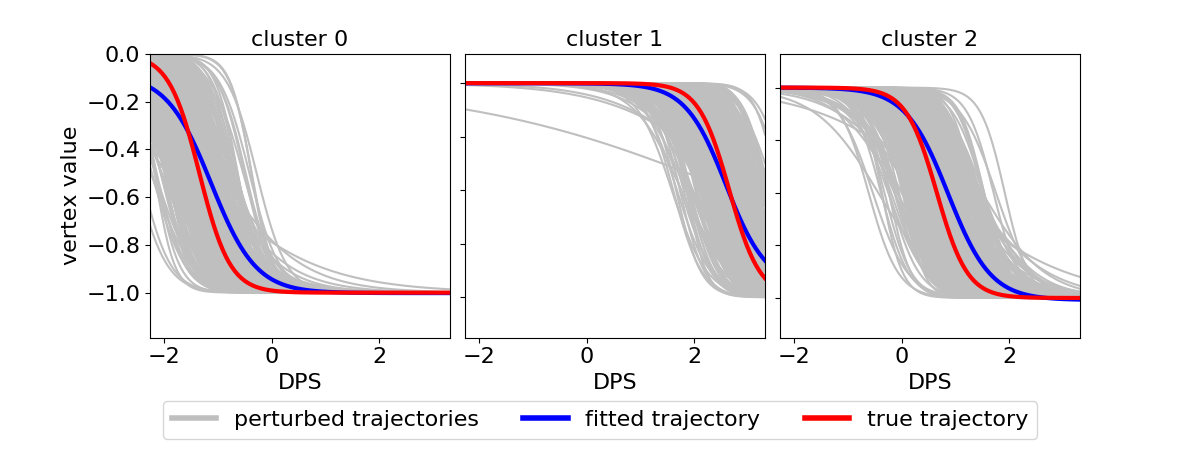
\includegraphics[width=1\textwidth,trim=30 0 60 0,clip]{\voxDpmFolder/resfiles/synth/trajCent0/initk-meansCl3Pr1Ra1_VWDPMMean/synThetaRes_initk-meansCl3Pr1Ra1_VWDPMMean.png}
\caption{}
\label{diveResSynthA}
\end{subfigure}
\begin{subfigure}[b]{0.25\textwidth}
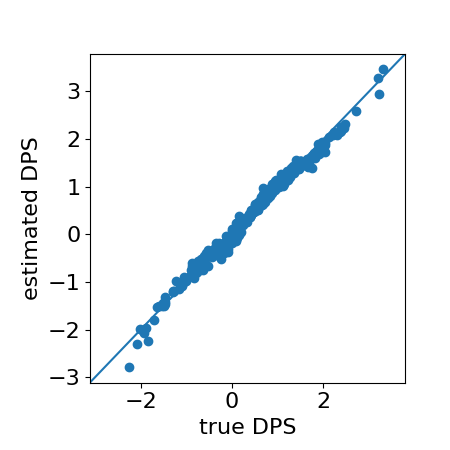
\includegraphics[width=1\textwidth,trim=0 0 0 0,clip]{\voxDpmFolder/resfiles/synth/trajCent0/initk-meansCl3Pr1Ra1_VWDPMMean/synShiftsRes_initk-meansCl3Pr1Ra1_VWDPMMean.png}
\vspace{0.4em}
\caption{}
\label{diveResSynthB}
\end{subfigure}
\begin{subfigure}[b]{0.32\textwidth}
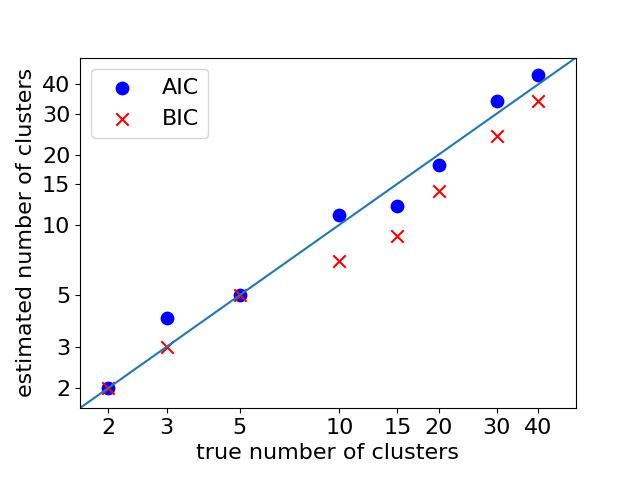
\includegraphics[width=1\textwidth]{\voxDpmFolder/resfiles/synth/nrClust.png}
\caption{}
\label{diveResSynthC}
\end{subfigure}
\begin{subfigure}[b]{0.32\textwidth}
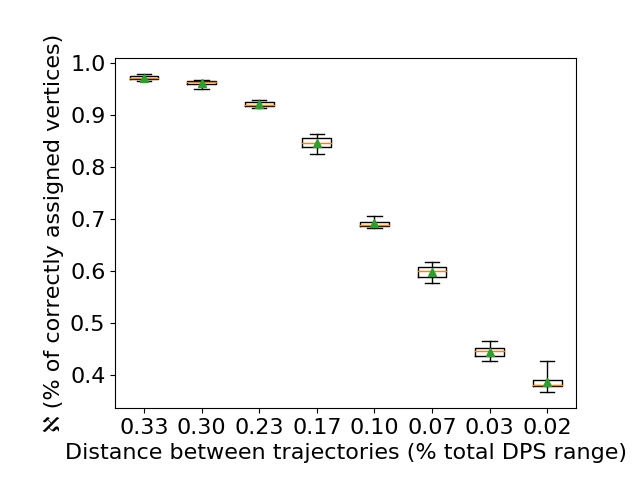
\includegraphics[width=1\textwidth]{\voxDpmFolder/resfiles/synth/correctVertices_trajCent.png}
\caption{}
\label{diveResSynthD}
\end{subfigure}
\begin{subfigure}[b]{0.32\textwidth}
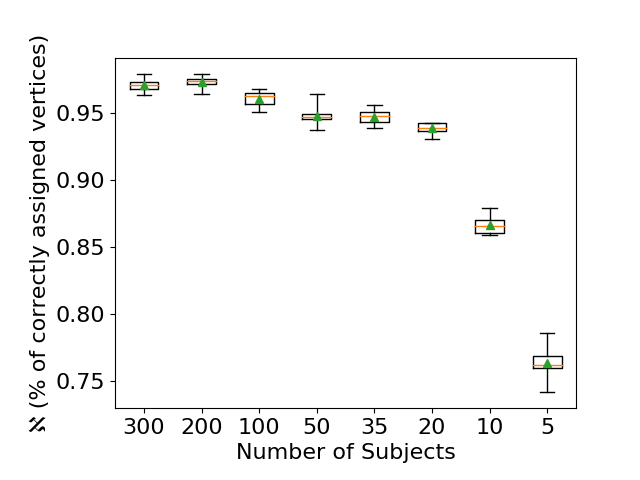
\includegraphics[width=1\textwidth]{\voxDpmFolder/resfiles/synth/correctVertices_nrSubj.png}
\caption{}
\label{diveResSynthE}
\end{subfigure}
\caption[DIVE Simulation Results]{(a-b) Results for the basic simulation, where trajectories are relatively well separated. (a) Reconstructed temporal trajectories (blue) plotted against the true trajectories (red). The x-axis shows the disease progression score (DPS), while the y-axis shows the biomarker values of the vertices. (b) Estimated subject-specific DPS scores compared to the true scores. (C-E) Simulation results for the three scenarios: (c) increasing number of clusters, (d) trajectories becoming similar and (e) decreasing number of subjects. On the x-axis we show the variable that was changing within the scenario (e.g. number of clusters), while on the y-axis we show the agreement measure $\aleph$, representing the percentage of vertices that were assigned to the correct cluster.}
\label{diveResSynth}
\end{figure}


\subsection{Results with ADNI and DRC Datasets}
\label{sec:diveResAdniDrc}

\subsubsection{Initial Hypotheses}

Using ADNI and DRC datasets, we aim to recover the spatial distribution of cortical atrophy and amyloid pathology, as well as the rate and timing of these pathological processes. In particular, we hypothesise that these spatial patterns of pathology and their evolution will be: 
\begin{itemize}
 \item similar on two independent typical AD datasets: ADNI and DRC
 \item different on distinct diseases: tAD vs PCA 
 \item different in distinct modalities: cortical thickness from MRI vs amyloid load from AV45 PET.
\end{itemize}

\subsubsection{Results}

The optimal number of clusters, as estimated with AIC, was three for the ADNI MRI dataset, three for the DRC tAD dataset, five for the DRC PCA dataset and eighteen for the ADNI PET dataset. Fig. \ref{diveClustAdniMri} (left) shows the results from the ADNI MRI dataset, where in the left image we coloured the vertices on the cortical surface according to the cluster they most likely belong to. We assigned a colour for each cluster (both the brain figures on the left and the trajectory figures on the right) according to the extent of pathology of its corresponding trajectory at a DPS score of 1. The cluster colours range from red (severe pathology) to blue (moderate pathology). In Fig. \ref{diveClustAdniMri} (right), we show the resulting cluster trajectories with samples from the posterior distribution of each $\theta_k$. Similar results are shown for the other three datasets: the DRC tAD dataset (Fig. \ref{diveClustDrcAd}), DRC PCA dataset (Fig. \ref{diveClustDrcPca}) and the ADNI PET dataset (Fig. \ref{diveClustAdniPet}).


We notice that in tAD subjects using the ADNI datasets (Fig. \ref{diveClustAdniMri}), there is more severe cortical thinning mainly in the inferior temporal lobe (red cluster), with disperse atrophy also in parietal and frontal regions (green cluster), with relative sparing of the inferior frontal and occipital lobes. In tAD subjects from the DRC dataset (Fig. \ref{diveClustDrcAd}), we see a relatively similar pattern, however with more pronounced atrophy in the supramarginal cortex (red cluster) compared to ADNI. This could be due to the younger ages of controls and tAD subjects in the DRC dataset as compared to ADNI. The spatial distribution of cortical thinning found with DIVE resembles results from previous longitudinal studies such as \cite{dickerson2008cortical,singh2006spatial}. However, in contrast to these approaches, our model gives insight into the timing and rate of atrophy and is also able to stage subjects across the disease time course. We also find that the cluster trajectories in the DRC tAD dataset have similar dynamics to the ADNI MRI dataset, although they show a clearer separation between each other.

In the PCA subjects (Fig. \ref{diveClustDrcPca}), we find that atrophy is mainly focused on the posterior part of the brain, with limited spread in the motor cortex, anterior temporal and frontal areas. This posterior-focused pattern of atrophy is different from the one found in the tAD datasets, and agrees with previous findings in the literature \cite{crutch2012posterior,lehmann2011cortical}.  However, as opposed to the results from \cite{lehmann2011cortical} which showed posterior regions uniformly affected, we notice that there are two clusters within the posterior region with different pathology dynamics, with the superior parietal and supramarginal areas affected more than the remaining posterior regions. This might be attributable to DIVE's ability to model subjects' disease onset and progression speed, along with non-linear cortical thinning dynamics, other differences due to the different subjects analysed, and the merging of left and right hemispheres could also give such differences.

In ADNI PET (Fig. \ref{diveClustAdniPet}) we see that the regions with the highest amyloid uptake are more spatially continuous, comprising the precuneus and anterior frontal areas. On the other hand, the anterior-superior temporal gyrus shows the least uptake of amyloid. This result closely matches the result by \cite{bilgel2016multivariate}, which used a completely different dataset and modelling technique. These results using AV45 PET are also noticeably different from results using cortical thickness (e.g. Fig. \ref{diveClustAdniMri}), which have more high-frequency patterns and only give 3-5 optimal clusters instead of 20. The “layers of clusters” starting from the precuneus and frontal lobes, which range from severe to less severe atrophy, suggest a continuum of variation in vertex trajectories in the case of the PET dataset (Fig \ref{diveClustAdniPet}, right). These trajectories all start with a low amyloid SUVR, between 0 and 0.25, but in late stages the trajectories for some clusters such as cluster 0 can reach an SUVR of 1.5. The reason for seeing this continuum might be because the PET images have a much lower resolution than MR images and were smoothed by ADNI during the pre-processing steps. 

\newcommand{\scalingFactor}{1.2}
\newcommand{\scalingFactorSubfigBrain}{0.35}

\newcommand{\gradLimLeft}{-1.6}
\newcommand{\gradLimRight}{1.6}

% \newcommand{\scalingFactorLeftFig}{1.2}
\newcommand{\scalingFactorBrains}{0.75}
\newcommand{\scalingFactorTraj}{1.05}

\newcommand{\typeOfBrainColoring}{atrophyExtent}

\definecolor{barGreen}{rgb}{0.4,1,0.4}

% FWHM0 avg thickness map MCI & AD
\begin{figure}
  \centering
  \vspace{-1em}

  % do the legend colorbar
  \begin{subfigure}[b]{0.45\textwidth}
   \centering
  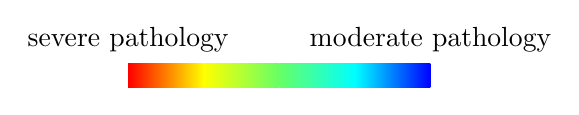
\begin{tikzpicture}[scale=\scalingFactor]
    \shade[left color=red,right color=yellow] (\gradLimLeft,2.5) rectangle (-0.8,2.75);
    \shade[left color=yellow,right color=barGreen] (-0.8,2.5) rectangle (0,2.75);
    \shade[left color=barGreen,right color=cyan] (0,2.5) rectangle (0.8,2.75);	
    \shade[left color=cyan,right color=blue] (0.8,2.5) rectangle (\gradLimRight,2.75);   
%     \node[inner sep=0] (corr_text) at (\gradLimLeft,2.25) {cluster 0};
%     \node[inner sep=0] (corr_text) at (0,2.25) {cluster 1};
%     \node[inner sep=0] (corr_text) at (\gradLimRight,2.25) {cluster 2};
    \node[inner sep=0] (corr_text) at (\gradLimLeft,3) {severe pathology};
    \node[inner sep=0] (corr_text) at (\gradLimRight,3) {moderate pathology};
  \end{tikzpicture}
%     \caption{}
%       \label{fig:adniClust}
  \vspace{1em}
  \end{subfigure}
  
  %%%%%%%%%%%%%%%%%%% BRAINS %%%%%%%%%%%%%%%%%%%%
  

  \begin{subfigure}[b]{\textwidth}
   \centering
  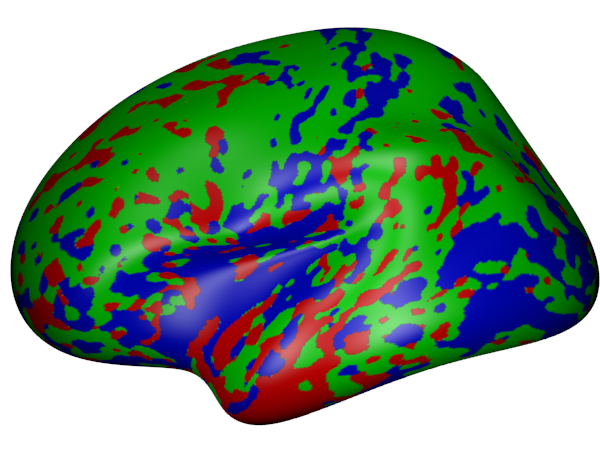
\includegraphics[width=\scalingFactorSubfigBrain \textwidth,trim=0 0 0 20,clip]{\voxDpmFolder/selected_resfiles/adniThick/atrophyExtent24_adniThInitk-meansCl3Pr1Ra1_VDPM_MRF.png} 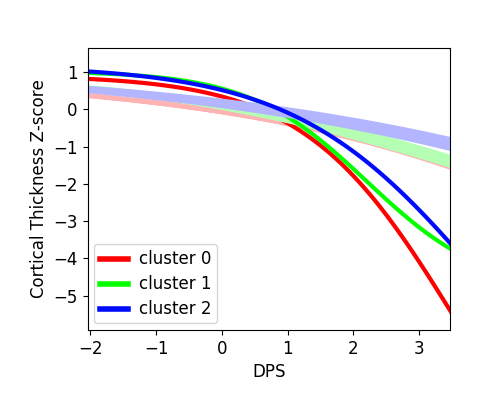
\includegraphics[width=\scalingFactorSubfigBrain \textwidth,trim=0 10 0 30,clip]{\voxDpmFolder/selected_resfiles/adniThick/trajSamplesOneFig_adniThInitk-meansCl3Pr1Ra1_VDPM_MRF.png}
    \caption{ADNI MRI}
    \label{diveClustAdniMri}
  \end{subfigure}

  \begin{subfigure}[b]{\textwidth}
   \centering
  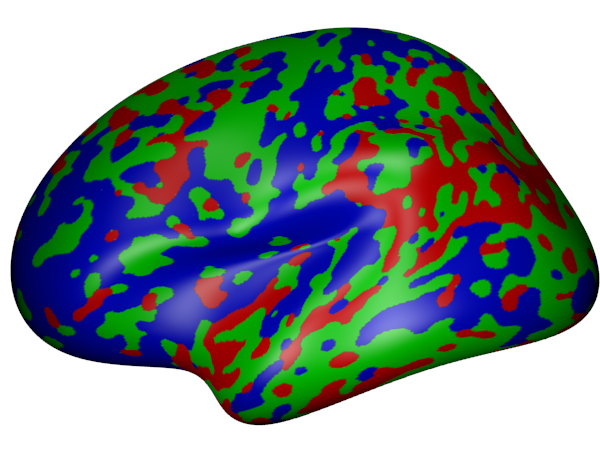
\includegraphics[width=\scalingFactorSubfigBrain \textwidth,trim=0 0 0 20,clip]{\voxDpmFolder/selected_resfiles/drcAD/atrophyExtent24_drcThInitk-meansCl3Pr1Ra1_VDPM_MRFAD.png} 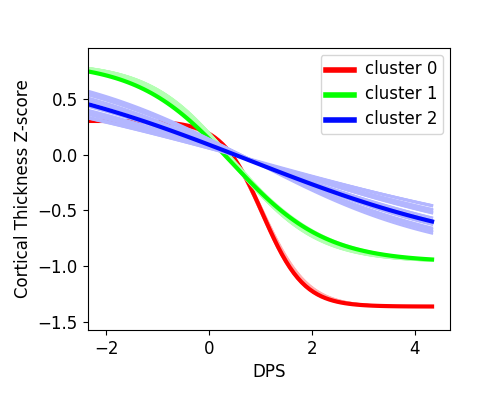
\includegraphics[width=\scalingFactorSubfigBrain \textwidth,trim=0 10 0 30,clip]{\voxDpmFolder/selected_resfiles/drcAD/trajSamplesOneFig_drcThInitk-meansCl3Pr1Ra1_VDPM_MRFAD.png}
    \caption{DRC tAD}
    \label{diveClustDrcAd}
  \end{subfigure}
  
  \begin{subfigure}[b]{\textwidth}
   \centering
  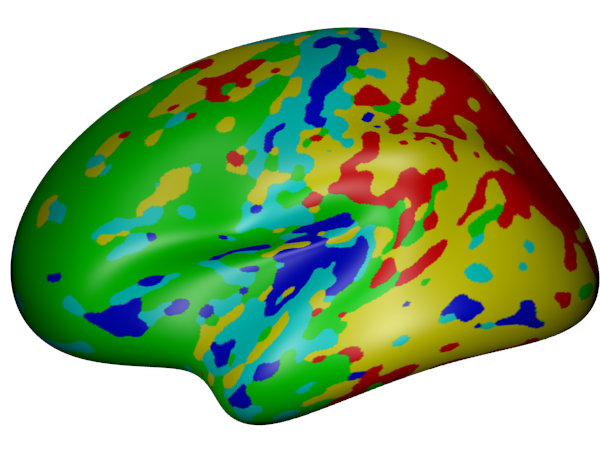
\includegraphics[width=\scalingFactorSubfigBrain \textwidth,trim=0 0 0 20,clip]{\voxDpmFolder/selected_resfiles/drcPCA/atrophyExtent24_drcThInitk-meansCl5Pr1Ra1_VDPM_MRFPCA.png} 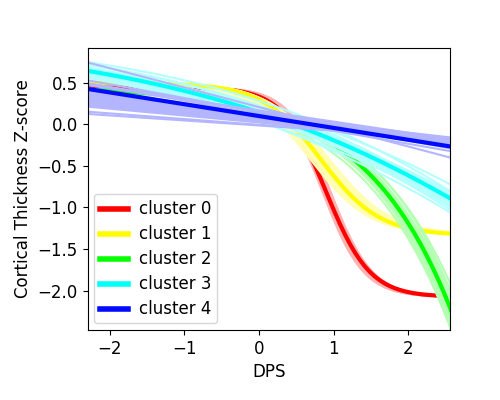
\includegraphics[width=\scalingFactorSubfigBrain \textwidth,trim=0 10 0 30,clip]{\voxDpmFolder/selected_resfiles/drcPCA/trajSamplesOneFig_drcThInitk-meansCl5Pr1Ra1_VDPM_MRFPCA.png}
    \caption{DRC PCA}
    \label{diveClustDrcPca}
  \end{subfigure}
  
  \begin{subfigure}[b]{\textwidth}
   \centering
  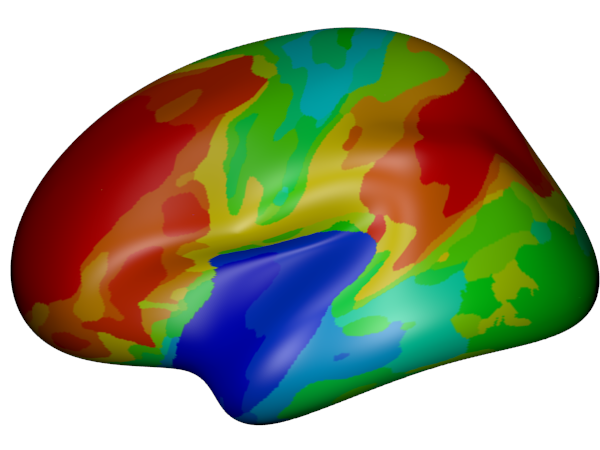
\includegraphics[width=\scalingFactorSubfigBrain \textwidth,trim=0 0 0 20,clip]{\voxDpmFolder/selected_resfiles/adniPet/atrophyExtent24_adniPetInitk-meansCl18Pr1Ra1_VDPM_MRF.png} 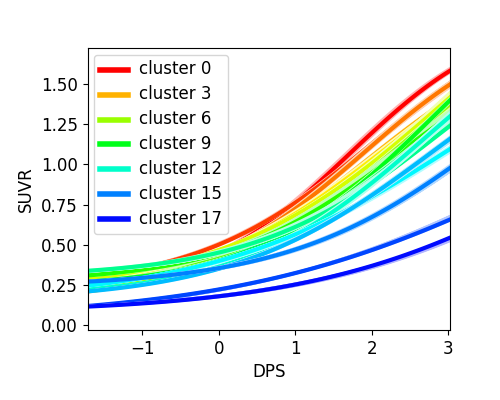
\includegraphics[width=\scalingFactorSubfigBrain \textwidth,trim=0 10 0 30,clip]{\voxDpmFolder/selected_resfiles/adniPet/trajSamplesOneFig_adniPetInitk-meansCl18Pr1Ra1_VDPM_MRF.png}
    \caption{ADNI PET}
    \label{diveClustAdniPet}
  \end{subfigure}
  
  %%%%%%%%%%%%%%%%%%%%%% trajectories %%%%%%%%%%%%%%%%%%%%%%%

  \caption[DIVE Results on ADNI and DRC cohorts]{(left column) DIVE estimated clusters (left column) and corresponding disease progression trajectories (right column) on four datasets: (a) ADNI MRI (b) DRC tAD (c) DRC PCA and (d) ADNI PET. We coloured each cluster according to the extent of pathology (cortical thickness or amyloid uptake) at DPS=1.}
  \label{diveClustTrajAll}
\end{figure}


\subsection{Model Evaluation}
\label{sec:diveEval}

\subsubsection{Motivation}
\label{sec:diveEvalMotiv}

We further tested the robustness and validity of the model as follows: 
\begin{itemize}
 \item Robustness in parameter estimation: test whether similar spatial clustering is estimated for different subsets of the data
 \item Clinical validity of DPS scores: test whether the subject disease progression scores, based purely on MRI or PET data, correlate with cognitive tests such as Clinical Dementia Rating Scale - Sum of Boxes (CDRSOB), Alzheimer's Disease Assessment Scale - Cognitive (ADAS-COG), Mini-Mental State Examination (MMSE) and Rey Auditory and Verbal Learning Test (RAVLT).
 \item Comparison with other models: to evaluate the benefit of estimating fine-grained patterns of pathology in DIVE, as well as latent time shifting of subjects, we compared the performance of DIVE with a region-of-interest based method \cite{jedynak2012computational} and a no-staging method that doesn't estimate subject time shifts. See Supplementary Section \ref{sec:diveCompAppendix} for precise specifications.
\end{itemize}


\subsubsection{Evaluation Procedure}

For all scenarios, we ran 10-fold cross-validation (CV) on the ADNI MRI dataset. At each fold we fit the model using 3 clusters, since this was the optimal number of clusters found previously on the entire dataset. The trained model was then used to estimate the DPS of the test subjects. 

For the performance comparison of DIVE with other models, we compute two performance metrics: (1) between-subject correlation of the models' estimated DPS values with cognitive tests; we estimated a unique DPS for every subject and every visit, which we then matched with the corresponding cognitive tests at that subject's visit and (2) prediction root mean squared error (RMSE) between the predicted vertex-wise values and actual measurements, averaged over all subjects and all locations on the brain; to evaluate these predictions, for every subject we use the first n-1 scans for training and the last scan for testing the prediction.


\subsubsection{Evaluation Results}


\newcommand{\outFoldADNICVbrains}{images/vwdpm/crossvalid/adniThavgFWHM0Initk-meansCl3Pr0Ra1_VWDPMMean}
\newcommand{\outFoldADNIPetCVbrains}{figures/validAdniPET/brainAtrophyExtent}

\newcommand{\adniThickCVExpName}{adniThInitk-meansCl3Pr1Ra1_VDPM_MRF}
\newcommand{\adniThickCVFolder}{\voxDpmFolder/resfiles/cogCorr/\adniThickCVExpName}
\newcommand{\trimModelValidTop}{0}

\begin{figure}
 \centering
\foreach \f in {0,1,2,3,4,5,6,7,8,9}
{
\begin{subfigure}[b]{0.185\textwidth}
\centering
  \FPeval{\faddOne}{clip(\f+1)}
  f = \faddOne \\
  \includegraphics[width=\textwidth, trim=0 0 0 \trimModelValidTop]{\adniThickCVFolder/f\f/atrophyExtent_cogCorr_\adniThickCVExpName_f\f.png}
\end{subfigure}
}
\vspace{1em}

 \begin{python}
for f in range(10): 
  if f == 5:
    print '\n'
  if f == 0 or f ==5:
    #print r''
    print r'\begin{subfigure}[b]{0.223\textwidth}'
    print r'\centering'
    print 'f=%d' % (f+1)
    print r'\includegraphics[width=\linewidth, trim=22 0 35 20,clip]{\adniThickCVFolder/'+ 'f%d/trajSamplesOneFig_cogCorr_\\adniThickCVExpName_f%d.png}' % (f, f)
    
  else:
    print r'\begin{subfigure}[b]{0.185\textwidth}'
    print r'\centering'
    print 'f=%d' % (f+1)
    print r'\includegraphics[width=\linewidth, trim=75 0 35 20,clip]{\adniThickCVFolder/'+ 'f%d/trajSamplesOneFig_cogCorr_\\adniThickCVExpName_f%d.png}' % (f, f)
  
  print r'\end{subfigure}%    <-- % added here'
  print r'\hfill'
\end{python}
\caption[DIVE estimated clusters and trajectories over the 10 cross-validation folds]{(top) Clusters estimated from 10-fold cross-validation training sets on the ADNI MRI dataset. (bottom) Estimated trajectories for each fold. }
\label{fig:diveClustTrajCV}
\end{figure}

Fig. \ref{fig:diveClustTrajCV} shows the brain clusters and corresponding trajectories, estimated for all the cross-validation folds after fitting the model on the training data. The clusters have been coloured using a similar colour scheme as in Fig. \ref{diveClustTrajAll}. In Fig \ref{fig:diveCogCorr} we show scatter plots of the DPS scores with clinical measures such as CDRSOB, ADAS-COG, MMSE and RAVLT.

\newcommand{\figFont}{\normalfont}
\newcommand{\pValFont}{\footnotesize}

\newcommand{\cogCorrScatterFold}{\voxDpmFolder/resfiles/adniThInitk-meansCl3Pr1Ra1_VDPM_MRF}

\begin{figure}[h]
  \begin{subfigure}{0.245\textwidth}
    \centering
    \hspace{1.5em}\figFont{CDRSOB}\\ 
    \hspace{1.5em}\pValFont{($\rho = 0.37$, $p < 1e-65$)}
    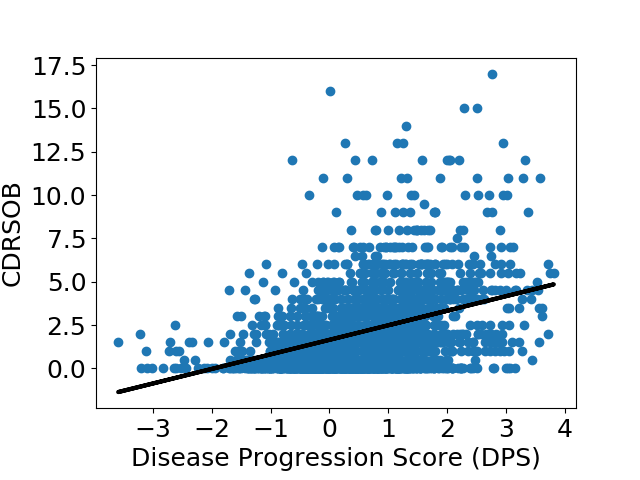
\includegraphics[width=1.1\textwidth]{\cogCorrScatterFold/stagingCogTestsScatterPlot_adniThInitk-meansCl3Pr1Ra1_VDPM_MRF_CDRSOB.png}
  \end{subfigure}
  \begin{subfigure}{0.245\textwidth}
    \centering
    \hspace{1.5em}\figFont{ADAS-COG}\\ 
    \hspace{1.5em}\pValFont{($\rho = 0.37$, $p < 1e-64$)}
    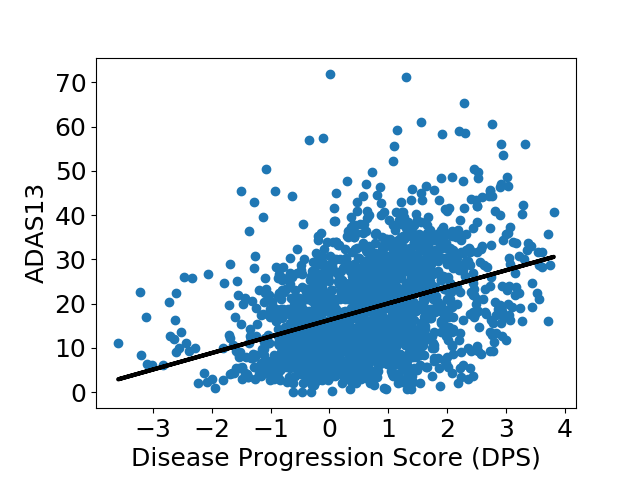
\includegraphics[width=1.1\textwidth]{\cogCorrScatterFold/stagingCogTestsScatterPlot_adniThInitk-meansCl3Pr1Ra1_VDPM_MRF_ADAS13.png}
  \end{subfigure}
    \begin{subfigure}{0.245\textwidth}
    \centering
    \hspace{1.4em}\figFont{MMSE}\\ 
    \hspace{1.4em}\pValFont{($\rho = -0.36$, $p < 1e-63$)}
    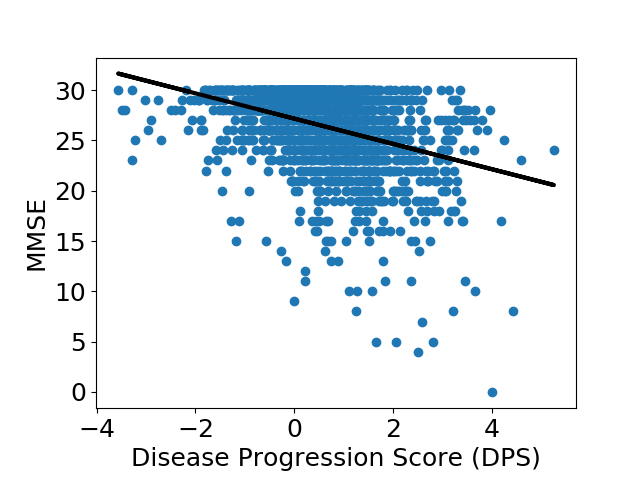
\includegraphics[width=1.1\textwidth]{\cogCorrScatterFold/stagingCogTestsScatterPlot_adniThInitk-meansCl3Pr1Ra1_VDPM_MRF_MMSE.png}
  \end{subfigure}
    \begin{subfigure}{0.245\textwidth}
    \centering
    \hspace{1.4em}\figFont{RAVLT}\\ 
    \hspace{1.4em}\pValFont{($\rho = -0.32$, $p < 1e-49$)}
    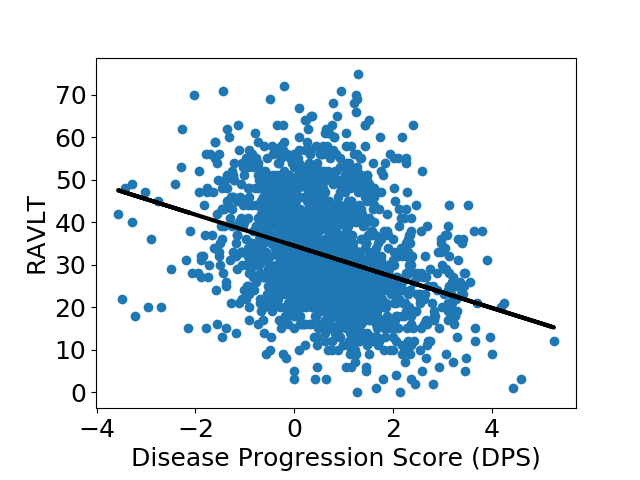
\includegraphics[width=1.1\textwidth]{\cogCorrScatterFold/stagingCogTestsScatterPlot_adniThInitk-meansCl3Pr1Ra1_VDPM_MRF_RAVLT.png}
  \end{subfigure}
  \caption[Scatter plot of DIVE-derived DPS scores vs cognitive tests]{Scatter plots of the DPS scores estimated from the ADNI MRI dataset, plotted against four cognitive tests: CDRSOB, ADAS-COG, MMSE and RAVLT. For each cognitive test we also report the Pearson correlation coefficient and p-value. The disease progression scores, computed only based on MRI cortical thickness data, correlate with these cognitive measures, suggesting that the DPS scores are clinically meaningful. }
  \label{fig:diveCogCorr}
\end{figure}



\begin{table}[H]
\centering
\begin{footnotesize}
 \begin{tabular}{c | c c c c | c}
  Model & CDRSOB ($\rho$) & ADAS13 ($\rho$) & MMSE ($\rho$) & RAVLT ($\rho$) & Prediction (RMSE)\\
  \hline 
DIVE & 0.37 $\pm$ 0.09 & 0.37 $\pm$ 0.10 & 0.36 $\pm$ 0.11 & 0.32 $\pm$ 0.12 & 1.021 $\pm$ 0.008 \\
ROI-based model & 0.36 $\pm$ 0.10 & 0.35 $\pm$ 0.11 & 0.34 $\pm$ 0.13 & 0.30 $\pm$ 0.13 & 1.019 $\pm$ 0.010 \\
No-staging model & *0.09 $\pm$ 0.06 & *0.03 $\pm$ 0.09 & *0.05 $\pm$ 0.06 & *0.02 $\pm$ 0.06 & *1.062 $\pm$ 0.024 \\

 \end{tabular}
 \end{footnotesize}
 \caption[Performance evaluation of DIVE and two simplified models on the ADNI MRI dataset]{Performance evaluation of DIVE and two simplified models on the ADNI MRI dataset using 10-fold cross-validation. In the middle four columns, we show between-subject correlations between the DPS scores and several cognitive tests: CDRSOB, ADAS-Cog13, MMSE and RAVLT. The last column shows the prediction error (RMSE) of cortical thickness values from follow-up scans. (*) Statistically significant differences between the model and DIVE, Bonferroni corrected for multiple comparisons.}
 \label{tab:divePerfEval}
\end{table}

The results in Fig. \ref{fig:diveClustTrajCV} demonstrate that DIVE is robust in cross-validation, as the estimated clusters and trajectory parameters are all similar across folds. The average Dice score overlap across the 10-folds range were 0.77, 0.76 and 0.90 for clusters 0, 1 and 2 respectively. The DIVE-derived DPS scores, which were estimated purely based on MRI data, are also clinically relevant as they correlate with cognitive tests (Fig. \ref{fig:diveCogCorr}). 

The performance of DIVE in terms of subject staging and biomarker prediction also compares favourably with simpler no-staging and ROI-based models (Table \ref{tab:divePerfEval}). Results show that DIVE has comparable performance to the ROI-based model, both in terms of subject staging and cortical thickness prediction. The fact that DIVE has similar performance to a simpler model which has less parameters is evidence that the estimated patterns are meaningful. Moreover, DIVE offers qualitative insight into the fine-grained spatial patterns of pathology and their temporal progression. Furthermore, the No-staging model performs significantly worse than DIVE, both in terms of subject staging and for biomarker prediction. This suggests that, when modelling progression of AD, it is important to account for the fact that patients are at different stages along the disease time-course.


\section{Discussion}
\label{sec:diveDis}

\subsection{Summary and Key Findings}

We presented DIVE, a spatiotemporal model of disease progression that clusters vertex- or voxel-wise measures of pathology in the brain based on similar temporal dynamics. The model highlights, for the first time, groups of cortical vertices that exhibit a similar temporal trajectory over the population. The model also estimates the temporal shift and progression speed for every subject. We applied the model on cortical thickness vertex-wise data from three MRI datasets (ADNI, DRC tAD and DRC PCA), as well as an amyloid PET dataset (ADNI). Our model found qualitatively similar patterns of cortical thinning in tAD subjects using the two independent datasets (ADNI and DRC). Moreover, it also found different patterns of pathology dynamics on two distinct diseases (tAD and PCA) and on different types of data (PET and MRI-derived cortical thickness). Finally, DIVE also provides a new way to parcellate the brain that is specific to the temporal trajectory of a particular disease, and enables staging of individuals at risk of disease, which can potentially help stratification in clinical trials.

The characteristics of the subjects' data used for training can affect the DIVE output. For instance, in cortical thinning analyses we standardised the data with respect to controls, which might have already shown cortical thinning due to early pathology. This can be mitigated through enrichment of the control population to amyloid-negative individuals. DIVE also relies on subjects spanning the entire disease progression, so inclusion of subjects in middle stages is recommended for a robust estimation of trajectories and spatial patterns. To reliably estimate the subject-specific time shift and progression speed, multiple follow-up scans are required. We mitigated this by using only subjects with at least three scans, and further placing informative priors on these parameters. 

The DIVE-estimated spatial patterns are patchier in MRI compared to PET scans, which had lower resolution and were smoothed a-priori. However, we believe MRI images should not instead smoothed a-priori, as the spatial correlation mechanism within DIVE enables it to automatically remove high-frequency patterns from MRI that are not meaningful.  Moreover, such a-priori smoothing could potentially loose dispersed patterns of pathology that arise due to underlying disruption of brain networks.



\subsection{Limitations and future work}

DIVE has some limitations that can be addressed. First, we assumed that cluster trajectories follow sigmoidal shapes, which is not the case for many types of biomarkers in ADNI which do not plateau in later stages. The assumption of sigmoidal trajectories can be avoided using non-parametric curves such as Gaussian Processes \cite{lorenzi2017disease}, which would be straightforward to incorporate into the DIVE framework. To get a reliable estimate of the subject-specific parameters, we only tested DIVE on balanced datasets, where subjects had at least three scans. However, DIVE can also be applied to less balanced datasets, by setting stronger priors on these parameters or even fixing the progression speed for every subject to 1. Another limitation of the model is that it assumes all subjects follow the same disease progression pattern, which might not be the case in heterogeneous datasets such as ADNI or DRC. This can be a concern, as there might be a pattern of pathology that occurs in a small set of subjects. However, DIVE can be extended to account for heterogeneity in the datasets by modelling subject-specific trajectories using random effects, or different progression dynamics for distinct subgroups, using unsupervised learning methods like the SuStaIn model by \cite{young2018uncovering}. While SuStaIn, just like DIVE, estimates clusters and trajectories within the dataset, the clusters in SuStaIn are made of subjects with similar disease progression, while the clusters in DIVE are made of vertices with similar progression. Future work could combine clustering along both subjects and vertices simultaneously to estimate disease subtypes with distinct spatiotemporal dynamics at the vertexwise level.

There are several potential future applications of DIVE. One of the advantages of DIVE is that it can be used to study the link between disconnected patterns of brain pathology and connectomes extracted from diffusion tractography or functional MRI (fMRI). Such an analysis would enable further understanding of the exact underlying mechanisms by which the brain is affected by the disease. Our model, which can estimate fine-grained spatial patterns of pathology, is more suitable than standard ROI-based methods for studying the link between pathology and these structural or functional connectomes, because white matter or functional connections have a fine-grained and spatially-varying distribution of endpoints on the cortex.

Apart from studying the link with brain connectomes, there are other potential applications for DIVE. While we only applied it to vertexwise data, the model can also be applied to study voxelwise data. Moreover, DIVE can be applied to other modalities or types of data, including FDG PET, tau PET, DTI or Jacobian compression maps from MRI. Moreover, the model can also be extended to cluster points on the brain surface according to a more complex disease signature, that can be made of two or more biomarkers. For example, using our cortical thickness and amyloid PET datasets from ADNI, we could have clustered points on the brain based on both modalities simultaneously. Such complex disease signatures can offer important insights into the relationships between different modalities and underlying disease mechanisms.

DIVE is a spatiotemporal model that can be used for accurately predicting and staging patients across the progression timeline of neurodegenerative diseases. The spatial patterns of pathology can also be used to test mechanistic hypotheses which consider AD as a network vulnerability disorder. All these avenues can help towards disease understanding, patient prognosis, as well as clinical-trials for assessing efficacy of a putative treatment for slowing down cognitive decline.

\section{Conclusion}
\label{sec:diveConclusion}

In this chapter I developed DIVE, a spatiotemporal model of disease progression that estimates fine-grained spatial patterns of brain pathology, while simultaneously placing subjects optimally on a disease time axis. I applied it to two typical AD MRI datasets (ADNI and DRC), one dataset of PCA patients, and one typical AD PET dataset. I also tested the robustness of the method in simulations, under cross-validation, and I've also compared its performance to simpler feature-based models.

In the next chapter, I will present another model, DKT, that can transfer information across different types of dementias in order to estimate the progression of rare dementias from limited, unimodal datasets. 
